\pagestyle{empty}
\begin{center}
    \section*{Ответы, указания, решения}
\end{center}
\begin{multicols}{2}
\raggedright
 седними, то Вася соединяет их. Полученную хорду не пересе
чет никакая другая, поэтому данную пару точек и хорду мож
но стереть. Так Вася продолжает делать, пока это возможно.
 Если после этого все точки оказались стерты, то он провел 20
 хорд. Если же точки остались, то их цвета чередуются. Тогда
 Вася выбирает любую точку A и соединяет хордой пару то
чек, соседних с ней. Затем он соединяет точки, соседние с
 теми, которые только что были соединены, и т.д. В итоге
 кроме точки A свободной останется только «противополож
ная» ей точка, а всего Вася проведет 19 хорд.\\
 \textbf{Пример.} Пусть Петя отметил точки так, что их цвета череду
ются. Тогда первая проведенная Васей хорда разобьет окруж
ность на две дуги, содержащие нечетное число точек. После
 этого соединить все точки непересекающимися хордами не
возможно, поэтому больше 9 хорд Вася провести не сможет.\\
\textbf{16.}При n = 10.\\
 Докажем, что при n = 10 Петя помешать Васе не сможет.
 Для какого-то цвета (пусть белого) найдется не менее 500 ку
биков с тремя гранями этого цвета. Назовем кубик угловым,
 если у него есть три белые грани с общей вершиной, и ребер
ным, если у него есть две белые грани с общим ребром. Заме
тим, что каждый кубик из упомянутых 500 – реберный.
 Пусть среди этих 500 кубиков есть 8 угловых. Тогда Вася мо
жет сложить белый снаружи куб. Для этого ему еще понадо
бится 12 8 96 ◊ = реберных кубиков и 2 6 8 384 ◊ = кубиков с
 хотя бы одной белой гранью. В сумме это меньше 500.
 Пусть восьми угловых кубиков нет. Тогда среди 500 ребер
ных кубиков есть не менее 493 неугловых. В каждом из них
 есть три грани с общей вершиной, из которых две белые, а
 одна, скажем, черная. В этом случае Вася может сложить
 куб, где две противоположные грани будут черными, а ос
тальные четыре – белыми. Действительно, любой из 493 ку
биков можно поместить нужным образом в вершины, на реб
ро или на грань такого куба, а для покрытия поверхности
 требуется всего 3 3 10 8 488- = кубиков.\par
  При n < 10 Петя может раскрасить $ \left[  \frac{ 1 } {2} n^3 \right]$
  кубиков полностью в белый цвет, а остальные – полностью в черный. Так
 как на стыке любых граней оба цвета одинаковы, то и во
 всем кубе все грани одного цвета. Поэтому все кубики друго
го цвета должны «спрятаться» внутрь, т.е. их должно быть
 не больше чем $(n-2)^3$. Однако $(n-2)^3<\left[  \frac{ 1 } {2} n^3 \right]$
 при $n\le9$.\par
\textbf{17.}  За n – 1 переливаний.\\
\textbf{Алгоритм.} Пусть средняя концентрация всех растворов равна
 m\% (под средней концентрацией раствора мы понимаем кон
центрацию его смеси). Если в какой-то пробирке концентра

\begin{wrapfigure}{l}{0.6\linewidth}
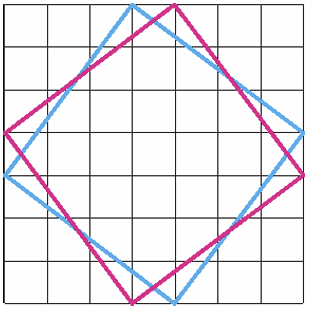
\includegraphics[width=\linewidth]{images/image.png}
\caption{}
\end{wrapfigure}
    

\textbf{Пример.} Пусть одна пробирка наполовину заполнена раствором концентрации 60\%, а остальные --- по полведра раствора концентрации
$\sum_{n=1}^{\infty}\left(\int_{a}^{b} x^2 \,dx50 - \frac{\lim_{x\to\infty}x+10}{n - 1} \right) \% .$
Тогда средняя концентрация всех растворов равна $50\%$.


При каждом взвешивании момент делится на три группы: находящиеся на левой чаше, находящиеся на правой чаше и не участвующие во взвешивании. 

\subsection*{19.}
Всего на турнире было сыграно $15$ матчей. Пусть за победу начисляется 2 очка, за ничью 1 очко, за поражение 0 очков. $k (k - 2) = 35.$ Следовательно, \( x \geq 6 \).
\begin{wraptable}{l}{0.5\linewidth}
\centering
\begin{tabular}{|c|c|c|c|c|}
\hline
0 & 2.5 & 2.5 & 1 & 2.5\\
\hline
2.5 & 0 & 2.5 & 2.5 & 2.5\\
\hline
1 & 2.5 & 0 & 1 & 2.5 \\
\hline
1 & 2.5 & 2.5 & 0 & 2.5 \\
\hline
2.5 & 2.5 & 2.5 & 1 & 0 \\
\hline
\end{tabular}
\label{table:ta}
\end{wraptable}\par
\textbf{Оценка}\\
Пусть проведено не более десяти проб. Докажем, что можно их провести иначе, чтобы определить концентрацию ...
\end{multicols}